\subsection{Datasets}\label{subsec:datasets}
There are many sources for csv or tsv files online that span a range of domains. We aim to test the proposed algorithm on a collection of data sets that vary in size and domain. Table \ref{tab:datasets} contains information on the characteristics of each data set. The runtimes stated are calcualted using the \textit{subset} \textit{NULL} interpretation in combination with \textit{duplicateAware} handling (see Section \ref{sec:null_subset}, Section \ref{sec:foundations}).

\begin{table*}[t]
    \centering
    \begin{tabular}{llrrrrrr}
        \hline
        \textbf{Name} & \textbf{Domain} & \textbf{Size on Disk} & \textbf{Relations} & \textbf{Attributes} & \textbf{Unaries} & \textbf{N-aries} & $\textbf{n}_\textbf{max}$ \\
        \hline
        Cars & Retail & 6.1 MB & 13 & 117 & 281 & 91 & 4 \\
        ACNH & Video-Games & 3.5 MB & 30 & 630 & 8,686 & 20,908,814 & 12 \\
        T2D & Benchmark & 4 MB & 669 & 3125 & 362,604 & 9,301,847 & 8 \\
        WebTables & Various & 5.3 MB & 5,000 & 18,663 & 19,924,741 & - & 1$^\dag$ \\
        US & Governmental & 1.2 GB & 16 & 255 & 753 & 215,308 & 7 \\
        EU & Governmental & 1.8 GB & 37 & 624 & 18,752 & 54,634 & 6 \\
        Population & Demographics & 1.7 GB & 1 & 109 & 236 & 1 & 2 \\
        Musicbrainz & Entertainment & 16.7 GB & 171 & 301 & 1,843 & 2,739,733 & 4$\dag$ \\
        UniProt & Biology & 633 MB & 263 & 2367 & 420,412 & 1,174,863 & 5 \\
        Tesma & Synthetic & 80 MB & 2 & 12 & 4 & 1 & 2 \\
        TPC-H 1 & Synthetic & 1 GB & 7 & 61 & 96 & 8 & 2 \\
        TPC-H 10 & Synthetic & 10.5 GB & 7 & 61 & 97 & 11 & 3 \\
        \hline
    \end{tabular}
    \caption{Datasets and their characteristics. Max n-ary layers marked with $^\dag$ are user defined limits.}
    \label{tab:datasets}
\end{table*}

\textbf{Cars} is a small dataset regarding used cars and their retail prices. The different relations each focus on a single brand (e.g. Audi, Ford or Skoda). Each row of a relation contains information on a specific model of that brand. The smallest dataset by required disk size, \textbf{ACNH}, contains data form the video game Animal Crossing: New Horizons\footnote{\url{https://animalcrossing.nintendo.com/new-horizons/} (Last Access: 30/06/2024)}. This dataset contains information on all items, recipes, and achievements in the game. It was selected since it contains a vast amount of deep (p)INDs a poses the challenge of efficient candidate handling. \textbf{T2D} is a gold standard for matching web tables to DBpedia\footnote{\url{https://www.dbpedia.org/} (Last Access: 30/06/2024)}. We use a subset of the 779 provided web table that span various domains. The subset includes all tables with at least five rows. Similar to \textbf{T2D}, \textbf{WebTables} offers an even larger collection. WebDataCommons published a random sample of their Web Table Corpus\footnote{\url{https://webdatacommons.org/webtables/2015/downloadInstructions.html} (Last Access: 30/06/2024)}. We use this sample to evaluate the capabilities when a massive amount of relations and attributes are present. We will not try to compute the n-ary pINDs for this data set. The \textbf{US} government and the European union (\textbf{EU}) both publicly share regional, national, and international data. The two dataset that are build on these sources represent the governmental domain. \textbf{Population} is a wide table containing world wide demographic data. It includes the population sizes for different ages in various countries from 1950, including predictions, up to 2025. \textbf{Musicbrainz} is a repository of music knowledge. The dataset in relational form has a large number of attributes, relations and rows. It is the most computational complex of the chosen datasets. The biological domain is covered by \textbf{UniProt}. This data set contains vertebrate genomes acquired from Ensembl \footnote{\url{https://www.ensembl.org/index.html} (Last Access: 30/06/2024)} in the UniProt\footnote{\url{https://www.uniprot.org/} (Last Access: 30/06/2024)} standard. Lastly, we have the synthetic datasets \textbf{Tesma} and \textbf{TPC-H}. \textbf{Tesma} is a database generation tool developed by the Hasso Plattner Institute. Using a configuration file with relational constraints and the desired size, it will create multiple csv files with the wanted structure. \textbf{TPC-H} is a benchmark for database performance. Using the generation tool, we have created a 1 GB version (\textbf{TPC-H 1}) and a 10 GB version (\textbf{TPC-H 10}). To enable reproducibility, the connected GitHub repository contains a detailed technical documentation on how each dataset was acquired\footnote{\url{https://github.com/Jakob-L-M/partial-inclusion-dependencies/tree/main/data} (Last Access: 30/06/2024)}.

\subsection{Hyperparameter Optimization}
There are five hyperparameters which influence the execution of \textit{SPIND}. The size of the initially created chunks (\textit{CHUNK}), the maximal number of values which are kept in main memory during the sorting phase per thread (\textit{SORT}), the maximal number of files which are merged at once per thread (\textit{MERGE}), the queue size for each relation during candidate validation (\textit{VALIDATION}) and the degree of parallelization (\textit{PARALLEL}). Leveraging Bayesian optimization \cite{shahriari2015taking}, we seek to efficiently and iteratively identify parameter configurations that minimize the execution time of \textit{SPIND} of various datasets. We lower bound \textit{CHUNK} by 10,000 to avoid the creation of a massive amount of files and set an upper bound of 100 million. We limit \textit{SORT} between 10,000 and 3.5 million to find a balance between a large number of files being written and a safe number under the main memory threshold. \textit{MERGE} is lower bounded by two and upper bounded by 1,000 to not put too much pressure on the file system. \textit{VALIDATION} is upper bounded by 1 million. Finlay, \textit{PARALLEL} is upper bounded by the number of virtual threads of the executing machine.

A first observation is that \textit{PARALLEL} has a clear negative correlation with the execution time. Regardless of how the other four parameters are set. Figure \ref{fig:parallelization_effectivness} shows a group of hex-bin plots, where the y-Axis is always the degree of parallelization and the x-Axis take on the other variables. After X?X iterations, our estimated multi-variable function has a maximal $2\sigma$ uncertainty of X?X. These observations lead to the decision of fixing \textit{PARALLEL} to its upper bound.

The next iteration yields that \textit{CHUNK} is the second most important variable. While smaller chunks strictly correlate with the total number of files being created and therefore also the I/O overhead, we find an optimum at a chunk size of five million which is robust over different datasets. A smaller chunk size enables more tasks to be processed in parallel which has been shown to overcome the I/O operations at some point.

Summarizing the last three iterations, we find that \textit{SORT} and \textit{VALIDATION} should be as large as possible under the given main memory constraints. The results for \textit{MERGE} X?X %TODO

In Figure \ref{fig:chunk_size} we can observe the relative change in the number of files created under changing chunk sizes (left) and the relative execution times compared to the longest run (right). For these experiments, we always average the execution of three runs.

\begin{figure}
    \centering
    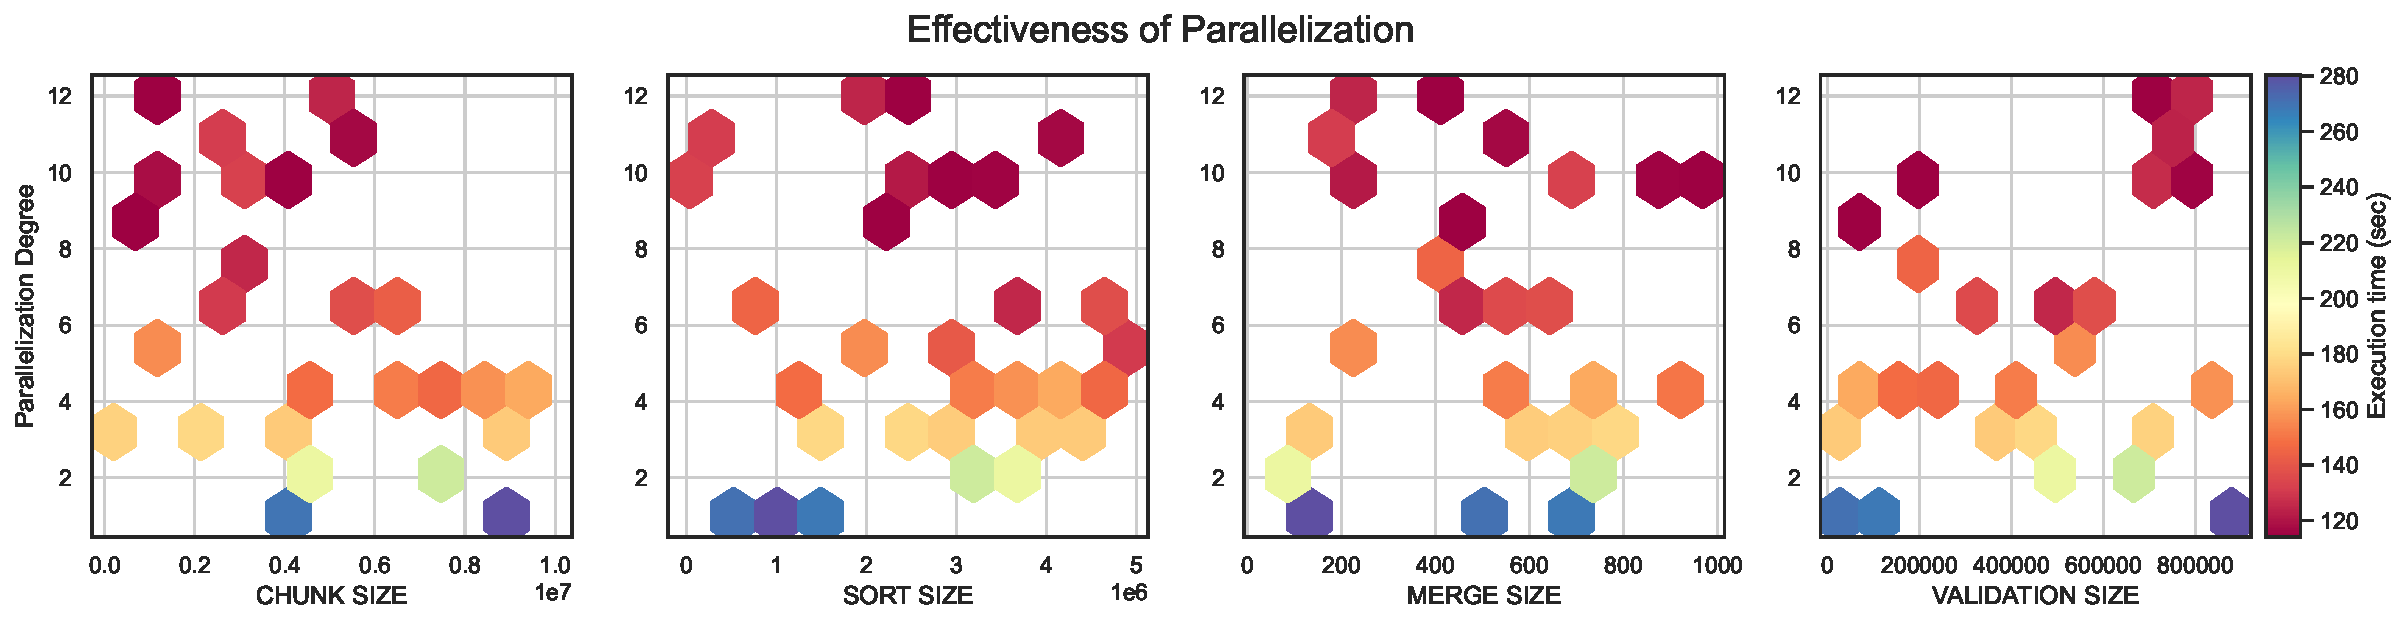
\includegraphics[width=.47\textwidth]{figures/parallelization.pdf}
    \caption{Effectiveness of the parallelization degree regardless of any other parameter.}
    \label{fig:parallelization_effectivness}
\end{figure}

\begin{figure}
    \centering
    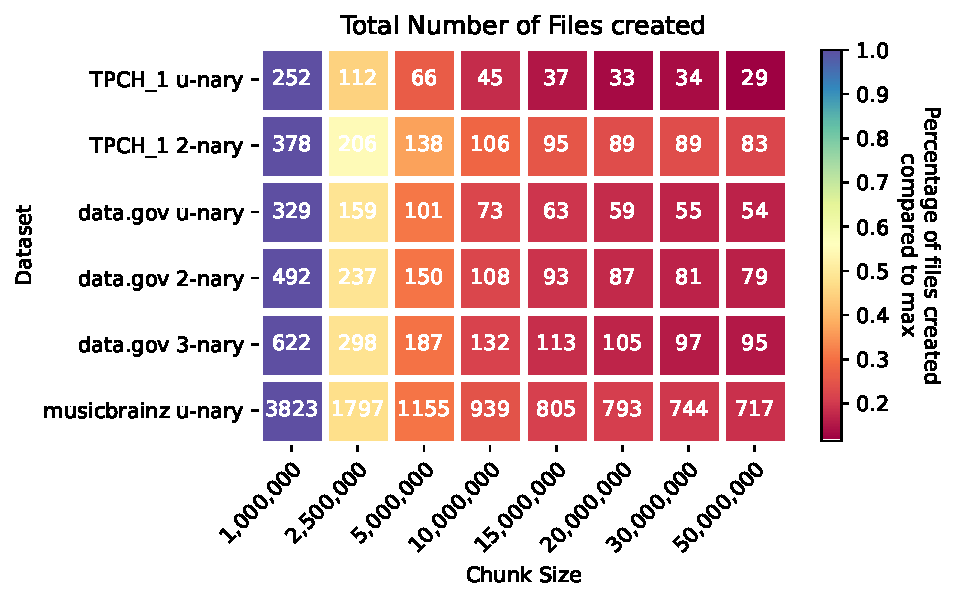
\includegraphics[width=.47\textwidth]{figures/chunk_size_files_created.pdf}
    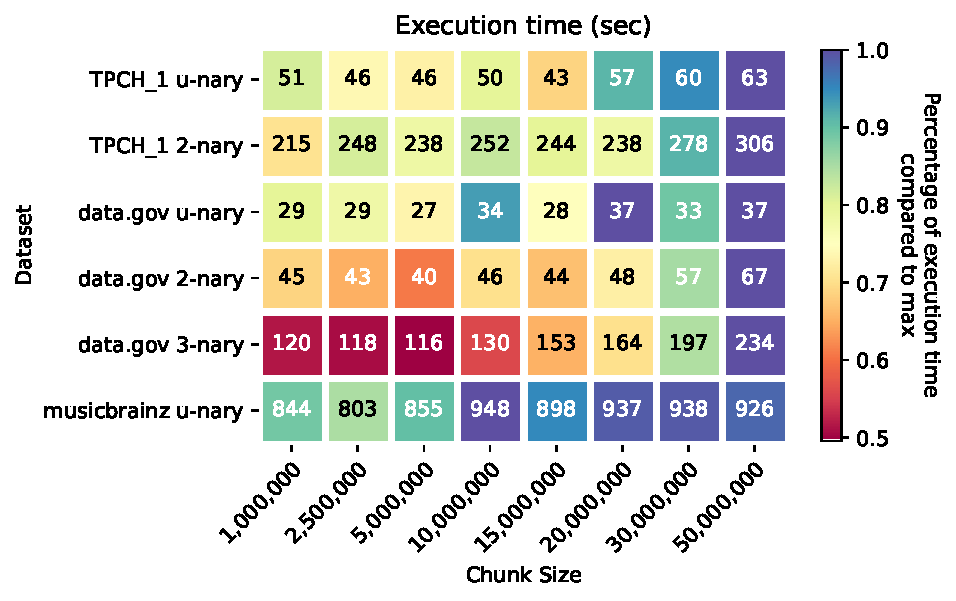
\includegraphics[width=.47\textwidth]{figures/chunk_size_execution_time.pdf}
    \caption{Files created (top) and execution time (bottom) under varying chunk sizes. Both relative to the maximum.}
    \label{fig:chunk_size}
\end{figure}

\subsection{Algorithm Runtimes} \label{subsec:runtime}
Table \ref{tab:runtimes} contains information on the total execution time of all data sets for the algorithms discussed for the discovery of unary and nary IND. All runs have been executed on the same machine, which is equipped with an AMD Ryzen 5 3600X, 32GB 3200MHz DDR4 RAM and dual Samsung 950 EVO SSDs. Each algorithm was limited to a maximal consumption of 20 GB RAM. We perform IND discovery to understand the execution times of the partial variants (\textit{pSPIDER}, \textit{pBINDER}, \textit{SPIND}) in comparison to known references (\textit{SPIDER}, \textit{BINDER}).

The memory overflow issue observed with the \textit{WebTables} dataset arises from \textit{SPIDER} employing HashMaps for candidate storage, which demands significantly more memory compared to using single linked lists. When discovering n-ary INDs, \textit{BINDER} did not finish the \textit{ACNH} and \textit{T2D} datasets. For \textit{ACNH} \textit{BINDER} was not able to finish the fourth layer in four hours and for \textit{T2D} the sixth layer could not be completed. In the case of \textit{ACNH} we can conclude that \textit{BINDER} was unable to complete $\sim18\%$ of the total candidates. When estimating the total run time using the growth of the attribute space in the deeper layers, we would expect \textit{BINDER} to take at least 24 hours, but most likely much longer due to poorer candidate generation. Using the same approximation, \textit{T2D} would also take over 24 hours. In addition, variants create millions of files and manually call the JVM garbage collector constantly, which causes execution to be very impractical. \textit{BINDER} and \textit{pBINDER} where also unable to finish \textit{Musicbrainz} within 12h. Both executions did not surpass the third layer while the second layer was completed after 5h 13m and 5h 4m respectively. \textit{SPIND} finished all data sets faster than the \textit{BINDER} variants. We find that data sets showing complex and deep (p)INDs are solved much faster by \textit{SPIND} while the ones with shallow (p)INDs can also be solved using \textit{BINDER} or \textit{pBINDER}.

When discovering unary INDs, we find \textit{pSPIDER} to present faster execution times. Parallelization and more efficient structures allow the algorithm to beat the original version by a factor of up to 14x (\textit{UniProt}). \textit{BINDER} and \textit{pBINDER} are able to narrow this factor, especially for larger data sets, but are still unable to beat \textit{pSPIDER} in any data set. \textit{SPIND} is structurally very similar to \textit{pSPIDER} when discovering unary INDs. Contrary to \textit{SPIND}, merging and validation are not performed at the same time, which causes \textit{SPIND} to take slightly longer while still outperforming the \textit{BINDER} variants.


\begin{table}[]
    \centering
    \resizebox{.475\textwidth}{!}{
        \begin{tabular}{lrrrrrr}
        \hline
        \textbf{Unary} & \textbf{\footnotesize SPIDER} & 
        \textbf{\footnotesize pSPIDER} &
        \textbf{\footnotesize BINDER} & 
        \textbf{\footnotesize pBINDER} &  
        \textbf{\footnotesize SPIND} \\
        \hline
        Cars & 1.1s & 0.5s & 1.3s & 1.3s & \textbf{0.2s} \\
        ACNH & 1.3s & 0.6s & 2.3s & 1.9s & \textbf{0.1s} \\
        T2D & 4.6s & 1.5s & 9.3s & 9.4s & \textbf{1.2s} \\
        WebTables & \textit{OOM} & \textbf{15.6s} & 1m 46s & 1m 19s & 16.0s \\
        US & 1m 58s & \textbf{14.0s} & 49.4s & 52.7s & 21.7s \\
        EU & 2m 5s & \textbf{21.3s} & 49.8s & 51.0s & 30.4s \\
        Population & 5m 36s & \textbf{34.4s} & 2m 36s & 2m 44s & 1m 32s \\
        Musicbrainz & 43m 20s & \textbf{10m 58s} & 24m 2s & 24m 41s & 12m 4s \\
        UniProt & 1m 43s & \textbf{7.0s} & 45.8s & 45.3s & 12.4s \\
        Tesma & 8.9s & \textbf{1.8s} & 3.8s & 4.2s & 3.8s \\
        TPC-H 1 & 2m 14s & \textbf{24.9s} & 55.1s & 53.4s & 38.1s \\
        TPC-H 10 & 27m 29s & \textbf{4m 57s} & 9m 19s & 9m 15s & 6m 10s \\
        \hline
        \hline
        \textbf{N-ary} & \textbf{\footnotesize SPIDER} & 
        \textbf{\footnotesize pSPIDER} &
        \textbf{\footnotesize BINDER} & 
        \textbf{\footnotesize pBINDER} &  
        \textbf{\footnotesize SPIND} \\
        \hline
        Cars & - & - & 2.8s & 2.8s & \textbf{1.5s} \\
        ACNH & - & - & \textit{DNF} & \textit{DNF} & \textbf{20m 35s} \\
        T2D & - & - & \textit{DNF} & \textit{DNF} & \textbf{33.3s} \\
        US & - & - & 3h 26m & 25min 39s & \textbf{2m 13s} \\
        EU & - & - & 2m 44s & 2m 23s & \textbf{44.0s} \\
        Population & - & - & 2h 40m & 2h 42m & \textbf{1h 58m} \\
        Musicbrainz & - & - & \textit{DNF} & \textit{DNF} & \textbf{2h 7m} \\
        UniProt & - & - & 7m 20s & 4m 25s & \textbf{25.1s} \\
        Tesma & - & - & 9.5s & 9.3s & \textbf{6.1s} \\
        TPC-H 1 & - & - & 4m 51s & 4m 40s & \textbf{4m 11s} \\
        TPC-H 10 & - & - & 56m 38s & 57m 3s & \textbf{47m 3s} \\
        \hline
    \end{tabular}
    }
    \caption{Runtime evaluation over the different datasets in both unary (top) and n-ary (bottom) settings. \textit{OOM}: Out of Memory, \textit{DNF}: Did not finish}.
    \label{tab:runtimes}
\end{table}

